La implementación final constó de dos bloques (Figura \ref{fig:implebloq}), uno de APLICACIÓN (Sección \ref{sec:aplic}) y otro de HARDWARE (Sección \ref{sec:hard}).
\begin{figure}[h!]
	\centering
	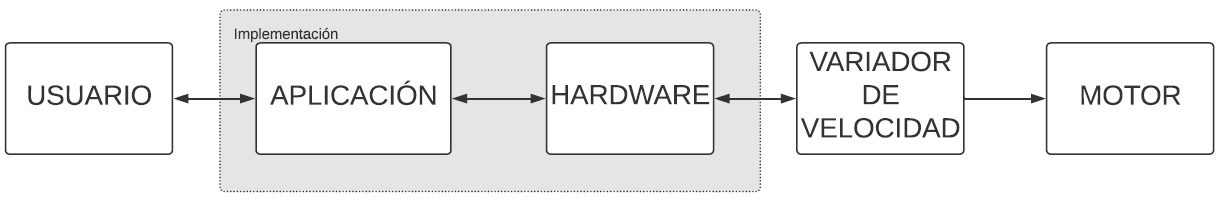
\includegraphics[scale=0.5]{bloqimplem.png}
	\captionof{figure}{Bloques implementados}
	\label{fig:implebloq}
\end{figure}





\subsection{Bloque Aplicación} 	\label{sec:aplic}
\begin{tcolorbox}[colback=blue!5!white,colframe=blue!75!black,title=GUI]
	La interfaz gráfica de usuario utiliza un conjunto de objetos gráficos para representar información y realizar acciones. El principal uso es un entorno de comunicación entre el usuario y algún elemento a controlar.
\end{tcolorbox}

Para la interfaz gráfica se creó un ejecutable para Windows, donde se utilizó el programa de código abierto \textit{Processing} en conjunto con la biblioteca \textit{ControlP5} \cite{controlp5}. La aplicación cuenta con comandos para configurar el funcionamiento del variador, configurar velocidades, realizar adquisición de datos y observar parámetros en tiempo real.
En el diagrama de flujo de la Figura \ref{fig:bloqvis} se observa que “aplicación” se divide en dos partes: 

\begin{figure}[H]
	\centering
	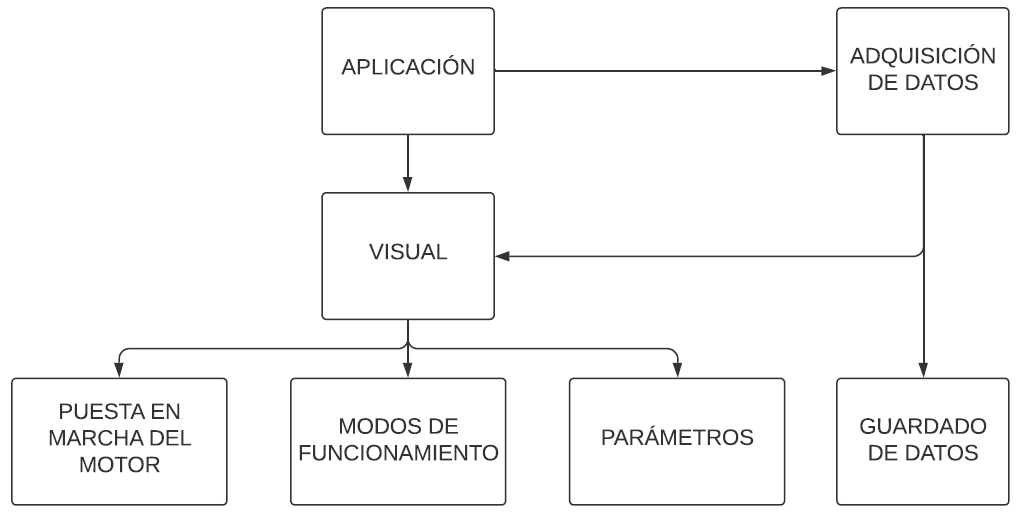
\includegraphics[scale=0.5]{aplibloques.png}
	\captionof{figure}{Bloque \textit{Aplicación}}
	\label{fig:bloqvis}
\end{figure}

\begin{enumerate}
\item Bloque \textbf{“Adquisición de datos”}: 
\subitem Obtiene datos provenientes del microcontrolador (Tabla \ref{tab:Datosdesde}) que son utilizados para guardar datos en un archivo “.csv”. 
\subitem Adquiere los datos que luego son utilizados por el bloque VISUAL.
 
Los datos que se reciben desde el microcontrolador durante el proceso de adquisición de datos consta de una cadena de caracteres en formato “string” dónde los distintos parámetros son separados por comas.
\begin{table}[H]
	\centering
	\begin{tabular}{|l|l|l|l|l|l|l|l|l|l|l|l|l|l|l|l|l|l|l|l|}
		\hline
		$D_0$ , & $D_1$ , & $D_2$ , & $D_3$ , & $D_4$ , & $D_5$ , & $D_6$ ,  & $D_7$ , & $D_8$ , & $D_9$ , & $D_{10}$ , & $D_{11}$ , & $D_{12}$ , & $D_{13}$ ,  \\ \hline
	\end{tabular}
\caption{Datos adquiridos desde el $u$C}
\label{tab:Datosdesde}
\end{table}

Referencia de cada dato:
	\begin{itemize}
	\item $D_0$: velocidad estimada utilizando THP y diferencia de presión.
	\item 	$D_1$: velocidad o frecuencia de referencia.
	\item 	$D_2$: diferencia de presión medida a través del MPX7002 en conjunto con ADS1115.
	\item 	$D_3$: señal de acción de control.
	\item 	$D_4$: tiempo otorgado por el microcontrolador.
	\item 	$D_5$: temperatura ambiente.
	\item 	$D_6$: humedad relativa del ambiente.
	\item 	$D_7$: presión atmosférica.
	\item 	$D_8$: densidad estimada por el microcontrolador.
	\item 	$D_9$: señal si se encuentra activado el control.
	\item 	$D_{10}$: error entre la velocidad estimada y la de referencia.
	\item 	$D_{11}$: estado encendido/apagado del motor.
	\item 	$D_{12}$: indicación de algún error del variador de velocidad.
	\item 	$D_{13}$: indicación de comienzo y fin del control automático.
	\end{itemize}	


\item Bloque \textbf{Visual}: 
\begin{itemize}
\item Sub-bloque \textbf{Parámetros}: con los datos adquiridos, muestra los valores de TPH, v y v/f ref y realiza gráficos en tiempo real donde el usuario decide la visibilidad de distintos parámetros (v, v/f ref, dDP, accion de control) y su correspondiente escala. 
\item Sub-bloque \textbf{Puesta en marcha del motor}: En el sub-bloque se encuentran botones de RUN y STOP que pondrán en marcha y pararán el motor según la configuración de F7 del variador de velocidad. En este bloque también se encuentran el botón de parada de emergencia y el botón de “Reset” ante alguna falla. 
\item Sub-bloque \textbf{Modos de funcionamiento}: posee las siguientes formas de ejecución del microcontrolador:
\begin{itemize}
\item \underline{Modo Lectura de datos:} al realizar la conexión del puerto serial, el microcontrolador comienza a adquirir datos, mostrando THP, velocidad y frecuencia de referencia por defecto. El modo solo recibe datos del microcontrolador pero esta configuración espera comandos de autofunción o del Modo Ai1 para enviar al microcontrolador una nueva orden.
\item \underline{Modo Autofunción:} El modo cierra el lazo de control, lee un archivo csv dónde se encuentran los escalones de velocidad y el tiempo de duración de estos. Envía al microcontrolador el archivo elegido, y este manda el comando para que se implementen los escalones establecidos.
\item \underline{Modo Ai1:} Este modo envía y recibe información del microcontrolador al variador, tiene dos funcionamientos
\begin{itemize}
\item Control desactivado: la planta se encuentra a lazo abierto y puede ser ingresada una frecuencia estimada.
\item Control activado: este método se utiliza como lazo de control cerrado, durante su funcionamiento se retroalimenta velocidad por lo que ante perturbaciones el sistema se establece en la velocidad de referencia configurada.
\end{itemize}
\end{itemize}
\end{itemize}


El formato de los datos enviados de la aplicación al microcontrolador es un vector de los datos separados por comas en formato “string” como se observan en la tabla \ref{tab:Datosenviados}, mientras que la referencia de cada elemento son:

\begin{table}[H]
	\centering
	\begin{tabular}{|l|l|l|l|l|l|l|l|l|l|l|l|l|l|l|l|l|l|l|l|}
		\hline
			$D_0$ , & $D_1$ , & $D_2$ , & $D_3$ , & $D_4$ , & $D_5$ , & $D_6$ ,  & $D_7$ , \\ \hline
	\end{tabular}
\caption{Datos enviados al $u$C}
\label{tab:Datosenviados}
\end{table}

\begin{itemize}
\item $D_0$: señal para que se encienda o se apague el motor desde la aplicación.
\item $D_1$: valor de velocidad o frecuencia de referencia.
\item $D_2$: señal para que el microcontrolador ingrese al modo “Ai1- Control activado”
\item $D_3$: señal para que el microcontrolador ingrese al modo “Ai1”
\item $D_4$: señal para que el microcontrolador se reinicie luego de alguna falla.
\item $D_5$: señal de falla externa que detiene el motor.
\item $D_6$: largo del vector ingresado por el archivo .csv.
\item $D_7$: vector de velocidades de referencias y tiempos de los escalones obtenidos del .csv.
\end{itemize}	

\end{enumerate}


\subsection{Bloque Hardware} \label{sec:hard}

Para llevar a cabo la implementación final del “hardware”, se procedió a realizar mediante el programa “Proteus” el diseño de una única placa uniendo los bloques anteriormente utilizados (Sección \ref{sec:desarr}) (Figura \ref{fig:hardBloq}). Esta nueva placa fue realizada por la máquina de prototipado \fcolorbox{red}{yellow}{“MARCA protomart”} perteneciente al Departamento de Electrónica de la Universidad. Una vez que se obtuvo la plaqueta se soldó componentes nuevos y se reutilizaron elementos utilizados durante la implementación del prototipo.  

\begin{figure}[H]
	\centering
	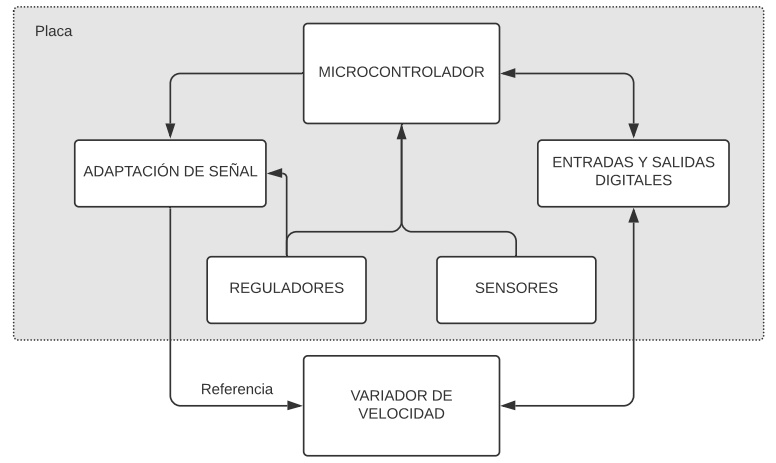
\includegraphics[scale=0.5]{placa_2.png}
	\captionof{figure}{Bloque \textit{Hardware}}
	\label{fig:hardBloq}
\end{figure}

En la \fcolorbox{red}{yellow}{figura WWW} se observa la placa terminada. Este nuevo prototipo elimina ruidos eléctricos ocasionados al utilizar cables para interconectar bloques y sensores.


\subsection{Costos}
El proyecto se comenzó a mediados del año 2019, por lo que los sensores de temperatura, humedad, 
presión atmosférica y diferencia de presión fueron comprados en esa fecha en el exterior y los demás componentes, en la actualidad, en la ciudad adaptándonos al stock encontrado. En la tabla \ref{gastos} se observan los valores totales para realizar la implementación final del \textit{hardware} con precios actualizados al mes de agosto de 2021. 


\begin{table}[H]
	\centering
	\begin{tabular}{|r|l|r|r|}
		\hline
		\multicolumn{1}{|c|}{\textit{\textbf{Unidad(es)}}} & \multicolumn{1}{c|}{\textit{\textbf{Descripción}}} & \multicolumn{1}{c|}{\textit{\textbf{Precio (\$)}}} & \multicolumn{1}{c|}{\textit{\textbf{Sub-Total  (\$)}}} \\ \hline
		1 & BME280 & 3850 & 3850 \\ \hline
		1 & MPXV7002dp & 8489 & 8490 \\ \hline
		1 & SI7021 & 3769 & 3770 \\ \hline
		10 & Resistencia 4.7k & 5 & 50 \\ \hline
		5 & Resistencia 10k & 5 & 25 \\ \hline
		5 & Resistencia 100k & 5 & 25 \\ \hline
		4 & Resistencia 20k & 7.5 & 30 \\ \hline
		2 & Resistencia 22k & 5 & 10 \\ \hline
		2 & Preset 1k & 180 & 360 \\ \hline
		1 & Preset 500 & 180 & 180 \\ \hline
		1 & Preset 10k & 180 & 180 \\ \hline
		1 & Diodo Zener 1N4740 (10V) & 25 & 25 \\ \hline
		1 & Diodo Zener 1N4001 & 15 & 15 \\ \hline
		2 & Capacitor 0.33uF & 35 & 70 \\ \hline
		2 & Capacitor 0.1uF & 15 & 30 \\ \hline
		1 & Capacitor 220uF-16V & 20 & 20 \\ \hline
		3 & Capacitor 10nF & 15 & 45 \\ \hline
		5 & Transistor BC548 & 30 & 150 \\ \hline
		1 & CI 74LS126 & 200 & 200 \\ \hline
		1 & CI LM358 & 70 & 70 \\ \hline
		1 & Borneras x2 & 180 & 180 \\ \hline
		1 & Borneras x3 & 200 & 200 \\ \hline
		1 & Fuente conmutada & 1500 & 1500 \\ \hline
		1 & Regulador 7810 & 180 & 180 \\ \hline
		1 & Regulador 7815 & 180 & 180 \\ \hline
		1 & ADC ADS1115 & 800 & 800 \\ \hline
		1 & Pines machos & 245 & 245 \\ \hline
		1 & Pines hembra & 245 & 245 \\ \hline
		1 & Arduino NANO & 900 & 900 \\ \hline
		\multicolumn{1}{|l|}{} & Caja contenedora & \multicolumn{1}{l|}{} & \multicolumn{1}{l|}{} \\ \hline
		\multicolumn{3}{|r|}{\textbf{Total=}} & \multicolumn{1}{c|}{\textbf{\$ 22025}} \\ \hline
	\end{tabular}
\caption{Gastos de implementación}
\label{gastos}

\end{table}

\subsection{Consumo de corriente}
NUEVA PLACA


\subsection{Planos eléctricos}
NOSE
